%!TEX program = xelatex
\documentclass[10pt]{article}
\usepackage{amssymb}
\usepackage{amsmath}
\usepackage{mathrsfs}
\usepackage{titlesec}
\usepackage{xcolor}
\usepackage{enumerate}
\usepackage{bm}
\usepackage{tikz}
\usepackage{listings}
\usetikzlibrary{arrows}
\usepackage{subfigure}
\usepackage{graphicx,booktabs,multirow}
\usepackage[a4paper]{geometry}
\usepackage{upquote}
\usepackage{float}
\usepackage{pdfpages}

\geometry{verbose,tmargin=2cm,bmargin=2cm,lmargin=2cm,rmargin=2cm}
\geometry{verbose,tmargin=2cm,bmargin=2cm,lmargin=2cm,rmargin=2cm}
\lstset{language=Matlab}
\lstset{breaklines}

\input defs.tex

\newtheorem{proposition}{Proposition}
\newtheorem{remark}{Remark}

\titleformat*{\section}{\centering\LARGE\scshape}
\renewcommand{\thesection}{\Roman{section}}
\lstset{language=Matlab,tabsize=4,frame=shadowbox,basicstyle=\footnotesize,
keywordstyle=\color{blue!90}\bfseries,breaklines=true,commentstyle=\color[RGB]{50,50,50},stringstyle=\ttfamily,numbers=left,numberstyle=\tiny,
  numberstyle={\color[RGB]{192,92,92}\tiny},backgroundcolor=\color[RGB]{245,245,244},inputpath=code}

\begin{document}

\date{\today}
\title{Introduction to Machine Learning, Fall 2023 \\
	Homework 1\\
	\small (Due Thursday, Oct. 26 at 11:59pm (CST))}
\maketitle
\begin{enumerate}[1.]


	\item
	\defpoints{10} [Math review] Suppose $\{\mathbf{X}_1, \mathbf{X}_2, \cdots, \mathbf{X}_n\}$ form a random sample from a multivariate distribution:
		\begin{itemize}
			\item[(a)] Prove that the covariance of $\mathbf{X}_i$ is a semi positive definite matrix. ~\defpoints{3}
			\item[(b)] Assuming $\mathbf{X}\sim \mathcal{N}(\mathbf{\mu},\mathbf{\Sigma})$ which is a multivariate normal distribution, and samples $X$, derive the the log-likelihood $\mathit{l}(\mathbf{\mu},\mathbf{\Sigma})$ and MLE of $\mathbf{\mu}$ ~\defpoints{4}
			\item[(c)] Suppose $\hat{\theta}$ is an unbiased estimator of $\theta$ and $\mathbf{Var}(\hat{\theta})>0$. Prove that $(\hat{\theta})^2$ is not an unbiased estimator of $\theta^2$. ~\defpoints{3}
		\end{itemize}
		
		\begin{enumerate}[(a)]
			\item 
			$$\mathbf{Cov}(X)=E[(X-E[X])^T(X-E[X])]$$
			Let $\vec a$ is a vector. Then 
			$$\vec a^T\mathbf{Cov}(X)\vec a=\vec a^TE[(X-E[X])^T(X-E[X])]\vec a=E[\vec a^T(X-E[X])^T(X-E[X])\vec a]=E[m^2]=\mathbf{Var}(m)>0$$
			$$\mbox{where }m=(X-E[X])\vec a$$
			$$\mbox{Therefore }\vec a^t\mathbf{Col}(X)\vec a>0$$
			Then, the covariance is a semi positive definite matrix.
			\item
			$$l(\mu,\Sigma)=\sum_{i=1}^N\log Pr_\theta(X_i)=\sum_{i=1}^N\log\frac{1}{(2\pi)^\frac N2|\Sigma|^\frac12}e^{-\frac{1}{2}(X_i-\mu)^T\Sigma^{-1}(X_i-\mu)}$$
			$$=-\log(2\pi)^\frac N2-\log|\Sigma|^\frac12-\sum_{i=1}^N\frac12(X_i-\mu)^T\Sigma^{-1}(X_i-\mu)$$
			$$\frac{\partial l(\mu,\Sigma)}{\partial\mu}=\frac{1}{\Sigma}\sum_{i=1}^N(X_i-\mu)=0\therefore\text{When }\mu=\frac{\sum_{i=1}^nX_i}{N}\text{, the log-likelihood has its maximum value}$$
			\item 
			Because $\hat\theta$ is unbiased, then we can say $\hat\theta=\frac1n\sum_{i=1}^n\hat\theta_i=E[\hat\theta]$
			
			Then, $\hat\theta^2=\frac{1}{n^2}\left(\sum_{i=1}^{n}\hat\theta_i\right)\neq\frac{1}{n}\sum_{i=1}^n\hat\theta^2=e{\hat\theta^2}$

			Then the $\hat\theta^2$ is not unbiased.
		\end{enumerate}
		\newpage

	\item \defpoints{10} Consider real-valued variables $X$ and $Y$, in which $Y$ is generated conditional on $X$ according to
	$$
	Y = aX + b + \epsilon, \ \text{where} \ \epsilon \sim \mathcal{N}(0, \sigma^2).
	$$
	Here $\epsilon$ is an independent variable, called a noise term, which is drawn from a Gaussian distribution with mean 0,
	and variance $\sigma^2$. This is a single variable linear regression model, where $a$ is the only weight parameter and $b$ denotes the intercept.
	The conditional probability of $Y$ has a distribution $p(Y | X, a, b) \sim \mathcal{N}(aX+b, \sigma^2)$, so it can be written as:
	$$
	p(Y|X, a,b) = \frac{1}{\sqrt{2\pi}\sigma}\exp\left(-\frac{1}{2\sigma^2}(Y - aX -b)^2\right).
	$$
	\begin{itemize}
		\item[(a)] Assume we have a training dataset of $n$ i.i.d. pairs $(x_i, y_i)$, $i = 1, 2, ..., n$, and
		the likelihood function is defined by $L(a,b) = \prod_{i=1}^n p(y_i | x_i, a, b)$. Please write the
		Maximum Likelihood Estimation (MLE) problem for estimating $a$ and $b$.~\defpoints{3}
		\item[(b)] Estimate the optimal solution of $a$ and $b$ by solving the MLE problem in (a).~\defpoints{4}
		\item[(c)] Based on the result in (b), argue that the learned linear model $f(X) = aX + b$,
		always passes through the point $(\bar{x},\bar{y})$,
		where $\bar{x} = \tfrac{1}{n}\sum_{i=1}^{n}x_{i}$ and $\bar{y} = \tfrac{1}{n}\sum_{i=1}^{n}y_{i}$ denote the sample means.~\defpoints{3}
	\end{itemize}
	\begin{enumerate}[(a)]
		\item 
		$$l(a,b)=\log L(a,b)=\sum_{i=1}^{n}\log Pr_\theta(y_i|x_i,a,b)=-\frac{1}{n}\log2\pi-n\log\sigma-\frac{1}{2\sigma^2}\sum_{i=1}^{n}(y_i-ax_i-b)^2$$
		Then find the minimum of $l(a,b)$
		\item 
		By the conclusion of 1(b), when $b=\frac{\sum_{i=1}^{n}y_i-a\sum_{i=1}^{n}x_i}{n}$, the MLE of $a,b$ get the maximum value.

		$$\frac{\partial l(a,b)}{\partial a}=\frac{1}{\sigma^2}\sum_{i=1}^{n}x_i(y_i-ax_i-b)=0$$
		$$\Rightarrow\sum_{i=1}^{n}(x_iy_i-ax_i^2-x_i\frac{\sum_{i=1}^{n}y_i-a\sum_{i=1}^{n}x_i}{n})$$
		$$\Leftrightarrow\sum_{i=1}^{n}x_iy_i-a\sum_{i=1}^{n}x_i^2-\frac{1}{n}\sum_{i=1}^{n}x_i\sum_{i=1}^{n}y_i+\frac{a}{n}(\sum_{i=1}^{n}x_i)^2=0$$
		$$\Leftrightarrow n\sum_{i=1}^{n}x_iy_i-\sum_{i=1}^{n}x_i\sum_{i=1}^{n}y_i=a\left(n\sum_{i=1}^{n}x_i^2-(\sum_{i=1}^{n}x_i)^2\right)$$
		$$\Leftrightarrow a=\frac{n\sum_{i=1}^{n}x_iy_i-\sum_{i=1}^{n}x_i\sum_{i=1}^{n}y_i}{n\sum_{i=1}^{n}x_i^2-(\sum_{i=1}^{n}x_i)^2}$$
		$$\Rightarrow b=\frac{\sum_{i=1}^{n}y_i-\sum_{i=1}^{n}x_i\frac{n\sum_{i=1}^{n}x_iy_i-\sum_{i=1}^{n}x_i\sum_{i=1}^{n}y_i}{n\sum_{i=1}^{n}x_i^2-(\sum_{i=1}^{n}x_i)^2}}{n}$$
		\item 
		Because $b=\frac{\sum_{i=1}^{n}y_i-a\sum_{i=1}^{n}x_i}{n}=\bar y-a\bar x$, therefore $\hat f(\bar x)=\hat a\bar x-\hat b=0$, which means the linear regression function always through the point $(\bar x,\bar y)$
	\end{enumerate}
	\newpage

	\item \defpoints{10} [Regression and Classification]
		\begin{itemize}
		\item[(a)] When we talk about linear regression, what does `linear' regard to? \defpoints{2}
		\item[(b)] Assume that there are $n$ given training examples $\{(x_1, y_1), (x_2, y_2), \cdots, (x_n, y_n)\}$,
		where each input data point $x_i$ has $m$ real valued features. When $m > n$, the linear regression model
		is equivalent to solving an under-determined system of linear equations $\mathbf{y} = \mathbf{X}\beta$. One popular way to
		estimate $\beta$ is to consider the so-called ridge regression:
		\[\argmin_{\beta} ||\mathbf{y}-\mathbf{X}\mathbf{\beta}||_2^2 + \lambda||\beta||_2^2\]
		for some $\lambda > 0$. This is also known as Tikhonov regularization.
		
		Show that the optimal solution $\beta_*$ to the above optimization problem is given by
		\[\mathbf{\beta}_* = (\mathbf{X}^T\mathbf{X} + \lambda \mathbf{I})^{-1}\mathbf{X}^T\mathbf{y}\]
		Hint: You need to prove that given $\lambda>0$, $\mathbf{X}^T\mathbf{X} + \lambda \mathbf{I}$ is invertible. \defpoints{5}
		\item[(c)] Is the given data set linear separable? If yes, construct a linear hypothesis function to separate the given data set. If no, explain the reason. \defpoints{3}
		
		\begin{table}[h]
			\centering
			\begin{tabular}{c|cccccc}
				Data & (1,3) & (4,4) & (3,-6) & (-2,1) & (-3,5) & (-6,-4) \\ \hline
				Label & +1 & -1 & -1 & +1 & -1 & -1
			\end{tabular}
			\label{tab:my_label}
		\end{table}
		\end{itemize}
		
		\begin{enumerate}[(a)]
			\item 
			The relation we supposed between $y$ and $x$ is linear, such as $y=ax+b$
			\item 
			$$\frac{\partial \argmin_\beta}{\partial \beta}=X^TX\beta+\lambda\beta-X^TY=0$$
			$$\text{By SVD decomposition, }X^TX=(U^TDV)^T(U^TDV)=(V^TDU)(U^TDV)=V^TD^2V$$
			$$\therefore X^TX+\lambda I=V^TD^2V+\lambda IV^TV=V^T(D^2+\lambda I)V$$
			$$\because I>0\therefore D^2+\lambda I\mbox{ is not a sigular matrix.}\therefore X^TX+\lambda I\mbox{ is invertible}$$
			$$\therefore\beta=(X^TX+\lambda I)^{-1}X^TY$$
			\item 
			We can draw the graph:

			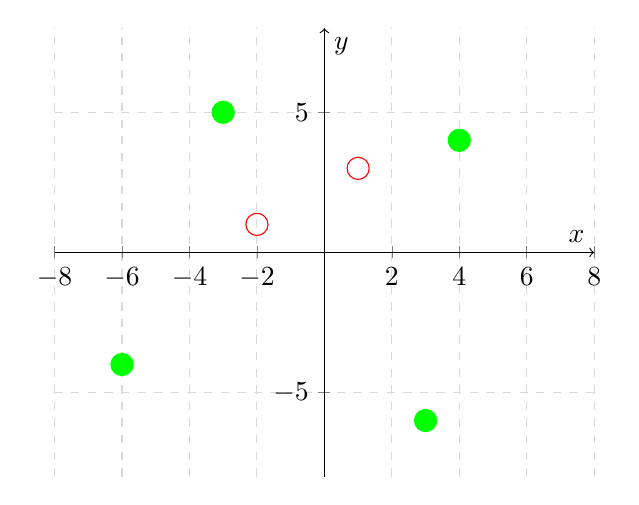
\begin{tikzpicture}
				\begin{axis}[
					xlabel=$x$,
					ylabel=$y$,
					axis lines=middle,
					axis line style={->},
					xmin=-8,
					xmax=8,
					ymin=-8,
					ymax=8,
					grid=both,
					grid style={dashed, gray!30},
				]
				
				% 红色点
				\addplot[only marks, mark=o, mark size=4pt, red] coordinates {
					(1,3)
					(-2,1)
				};
				
				% 绿色点
				\addplot[only marks, mark=*, mark size=4pt, green] coordinates {
					(4,4)
					(3,-6)
					(-3,5)
					(-6,-4)
				};
				\end{axis}
				\end{tikzpicture}

				So we can easily know that we can not given a linear separable.
		\end{enumerate}

		\newpage


\end{enumerate}

\end{document}